\documentclass[main.tex]{subfiles}
\begin{document}

\chapter*{Bilag 1 - Dysfagi}
\label{Bilag1}
\section*{Indledning}
Når man drikker eller og spiser skal dette forbi svælget og videre ned i spiserøret. Denne synkningsprocess foregår ved at den tygget mad skubbes bagud mod svælget, ved hjælp af tungen som presser op og bagud. Nu udløses en refleks pga. sanseceller i svælget. Dette foregår uden for viljens kontrol og i forbindelse med den forlængede rygmarv. Hele synkeprocessen er et samspil mellem 20-30 muskler som enten skal trække sig sammen eller slappe af i den rigtige rækkefølge. \cite{Sand2008MennesketsFysiologi}

Synkeprocessen består af tre sammenhængende faser:\cite{Bass1992Dysphagia:Management}
\begin{enumerate}
\item Oral fase (i munden)\\
I den første fase bliver maden bidt i stykker og ført i munden. Nu tykkes maden som bliver blandet med spyt og formet til en bolle (bolus). Ved hjælp af tungen transporteres bolus til den bagerste del af mundhulen samtidig med at ganespejlet lukker af op til næsen.
\item Faryngeale Fase (i svælget)\\
Nu kommer maden fra mundhulen og ned i svælget, ved at der synkes. 
\item Esophageal Fase (i spiserøret)
\end{enumerate}

\begin{figure}[H]
\centering
{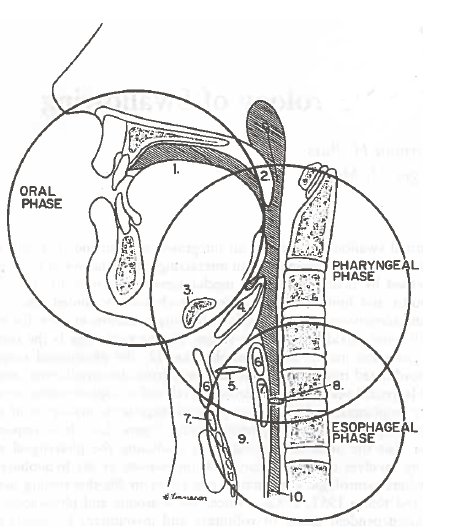
\includegraphics[width=8cm]
{Figure/dysfagi3faser}}
\caption{De tre faser ved synkeprocessen\cite{Bass1992Dysphagia:Management}}
\label{trefaser}
\end{figure}


\section*{Hvad er dysfagi?}
Dysfagi er når man har problemer med at tygge og synke mad og drikke. Dysfagi opstår når man ikke får lavet en korrekt synkning, men får lavet en fejlsynkning. I stedet for bolus ender i spiserøret går det i stedet går ned i luftvejene, så man risikere at få det galt i halsen og resultere i bl.a. lungebetændelse. Dysfagi findes i patientgrupper som eksempel sklerose, hjerneskade eller parkinson. Dog forekommer det også ved kræft, KOL eller almen svækkelse og aldring.\cite{SallyRefsgaardTinesterbyKristensen2015DysfagiKommune}

Dysfagi kan have følgende konsekvenser:
\begin{itemize}
\item Lungebetændelse
\item Dårlig ernæringstilstand
\item Væskemangel
\item Vægttab
\item nedsat livskvalitet
\item Social isolering

\end{itemize}






\section*{Hvor opstår dysfagi? anatomi}

\nameref{Bilag1}

\section*{Hvor opstår dysfagi? sygdommen?}

Diagnosticering af øvre dysfagi kan inddeles i tre faser. Den første fase handler om at screene patientens mentale tilstand ved at vurdere patientens bevidsthedsniveau, orienteringsevne, handlekraft, samt evnen til at synke få konsistenstyper som vand og spytflåd. Hvis det vurderes af klinikeren at der er behov for yderligere udredning, sendes patienten videre til næste undersøgelsesfase som er en klinisk undersøgelse. Den kliniske undersøgelse er baseret på Facial-Oral-Tract-Therapy (F.O.T.T) metoden og anvendes til at vurdere parametre som patientens sensoriske/motoriske respons, åndedræt og oral indtagelse af fødebolus \cite{Kjaersgaard2013PhDPerspective}. Den kliniske undersøgelse er en subjektiv undersøgelse, da det foretages af en klinikker uden hjælp af teknologisk apparater. Denne undersøgelsesmetode mangler præcision til f.eks. at opdage silent aspiration, som kan medføre udvikling lungebetændelse og i værste fald kvælning. Derfor anbefales det af sundhedsstyrelsens nationale klinisk retningslinjer for øvre dysfagi at man supplere den kliniske undersøgelse med en instrumentel undersøgelse til voksne med synkebesvær \c
Den instrumentelle undersøgelse omfatter Fiber Endoskopisk Evaluering af Synkefunktionen (FEES) og/eller Funktionel Videoradiologisk Evaluering af Synkefunktionen (FVES).  Ved FEES undersøgelse, som er en invasiv intervention, fører klinikeren en fiberoptisk endoskop gennem patientens næse og pharynx/svælget for at få et visuelt billede af svælgets anatomi. Anormaliteter, som observeres undervejs dokumenteres i en modificeret udgave af ”Der Berliner Dysphagia Index” som er en standard protokol til dokumentation af FEES undersøgelse . Undersøgelsen kan afdække patientens synkevanskeligheder ved at iagttage aspiration af bolus i luftvejene, tilstedeværelsen af bolus-rester i strubehovedet og patientens evne til at synke egen saliva . 
Ved FVES undersøgelse anvendes røntgenstråler, som muliggør visualisering af fødebolus i alle faser. Klinikeren kan vha. denne metode evaluere om pharyngeal eller esophageal muskler fungerer korrekt og om patienten kan kompensere for dysfagien med reflektoriske teknikker som ændring af hovedstilling. FEES og FVES anvendes som ”guld standarder” ved diagnosticering af patienter med øvre dysfagi, og begge undersøgelsesmetoder betragtes som komplementære værktøjer til udredning af dysfagi frem for konkurrerende .



\bibliography{Mendeley.bib}
\end{document}